\documentclass[handout]{beamer}
\usepackage[utf8]{inputenc}
\usepackage{graphics}
\mode<presentation> {
\usetheme{unc}}
\setbeamertemplate{navigation symbols}{} % To remove the navigation symbols from the bottom of all slides uncomment this line

\usepackage{graphicx} % Allows including images
\usepackage{booktabs} % Allows the use of \toprule, \midrule and \bottomrule in tables


\usepackage{hyperref}
\hypersetup{linkcolor=blue,colorlinks=true}


% Remove symbols
\beamertemplatenavigationsymbolsempty


%\usetheme{default}

\usefonttheme{serif}

%----------------------------------------------------------------------------------------
%	TITLE PAGE
%----------------------------------------------------------------------------------------


\title[Terrorism]{\LARGE{Terrorism and Counter-Terrorism}}
\author[POLI 150]{Steven Saroka}
\institute{POLI 150}
\date{27 February 2024}


\begin{document}

\begin{frame}
\titlepage % Print the title page as the first slide
\end{frame}



%----------------------------------------------------------------------------------------
%	PRESENTATION SLIDES
%----------------------------------------------------------------------------------------

	\begin{frame} 
	\frametitle{\LARGE{Announcements}}
	\begin{itemize}
		\item NO CLASS Feb. 29.
		\item Subject pool module 1 now open until Mar. 6. 
		\item Exam 1 on March 7.
		
	\end{itemize}
\end{frame}

\begin{frame} 
\frametitle{\LARGE{Today's Class}}
	\begin{itemize}
		\Large{
			\item Definition of Terrorism
			\\~\\ 
			\item Terrorism and Strategic Actors
			\\~\\
			\item Types of Terrorism
			\\~\\
			\item Effectiveness of Terrorism
			\\~\\
			\item Counter-terrorism Strategies
		}
	\end{itemize}
\end{frame}

\begin{frame} 
	\frametitle{\LARGE{Key Terms}}
	\begin{itemize}
		\item Terrorism (domestic and international)
		\item Elements of terrorism
		\item Terrorism tactics
		\item Counterterrorism tactics
	\end{itemize}
\end{frame}

\begin{frame} 
	\frametitle{\LARGE{Central Question}}
    \centering
    \Large{What is terrorism and why do political actors use it?} 
\end{frame}

%Source:  https://www.reuters.com/news/picture/defining-images-from-the-9-11-attacks-idUSRTXGV6X0

\begin{frame} 
	\frametitle{\LARGE{Terrorism}}
	\begin{figure}[ht!]
		\centering
		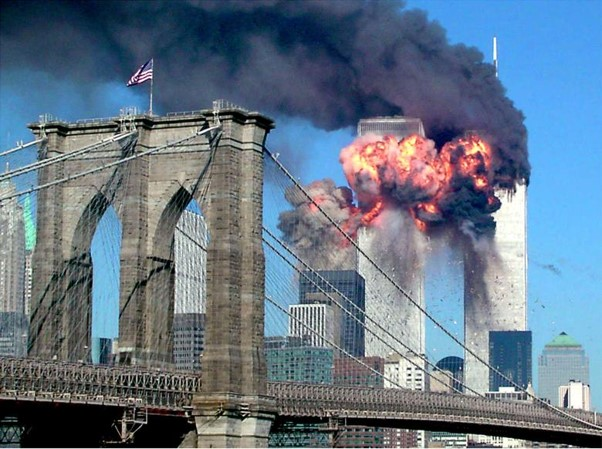
\includegraphics[width=\textwidth,height=.9\textheight,keepaspectratio]{911.jpg}
	\end{figure}
\end{frame}

\begin{frame} 
\frametitle{\LARGE{What is Terrorism?}}
\textbf{Terrorism has a multi-part definition:}
\begin{itemize}
		\item Premeditated threat or use of violence \pause
		\item against noncombatant targets \pause
		\item by individuals or nonstate actors \pause
		\item for the purpose of influencing a group larger than the immediate victims.
\end{itemize}
\end{frame}

\begin{frame} 
	\frametitle{\LARGE{What is Terrorism?}}
All terrorism is either:
	\begin{itemize}
		\item \textbf{Domestic}: involving perpetrators and victims from the same state. \pause
		\item \textbf{International}: involves perpetrators and victims from different states and/or is intended to alter a foreign state's behavior. \pause
	\end{itemize}
Empirically, what does terrorism look like?
\end{frame}

\begin{frame} 
	\frametitle{\LARGE{Terrorism in 2020}}
	\begin{figure}[ht!]
		\centering
		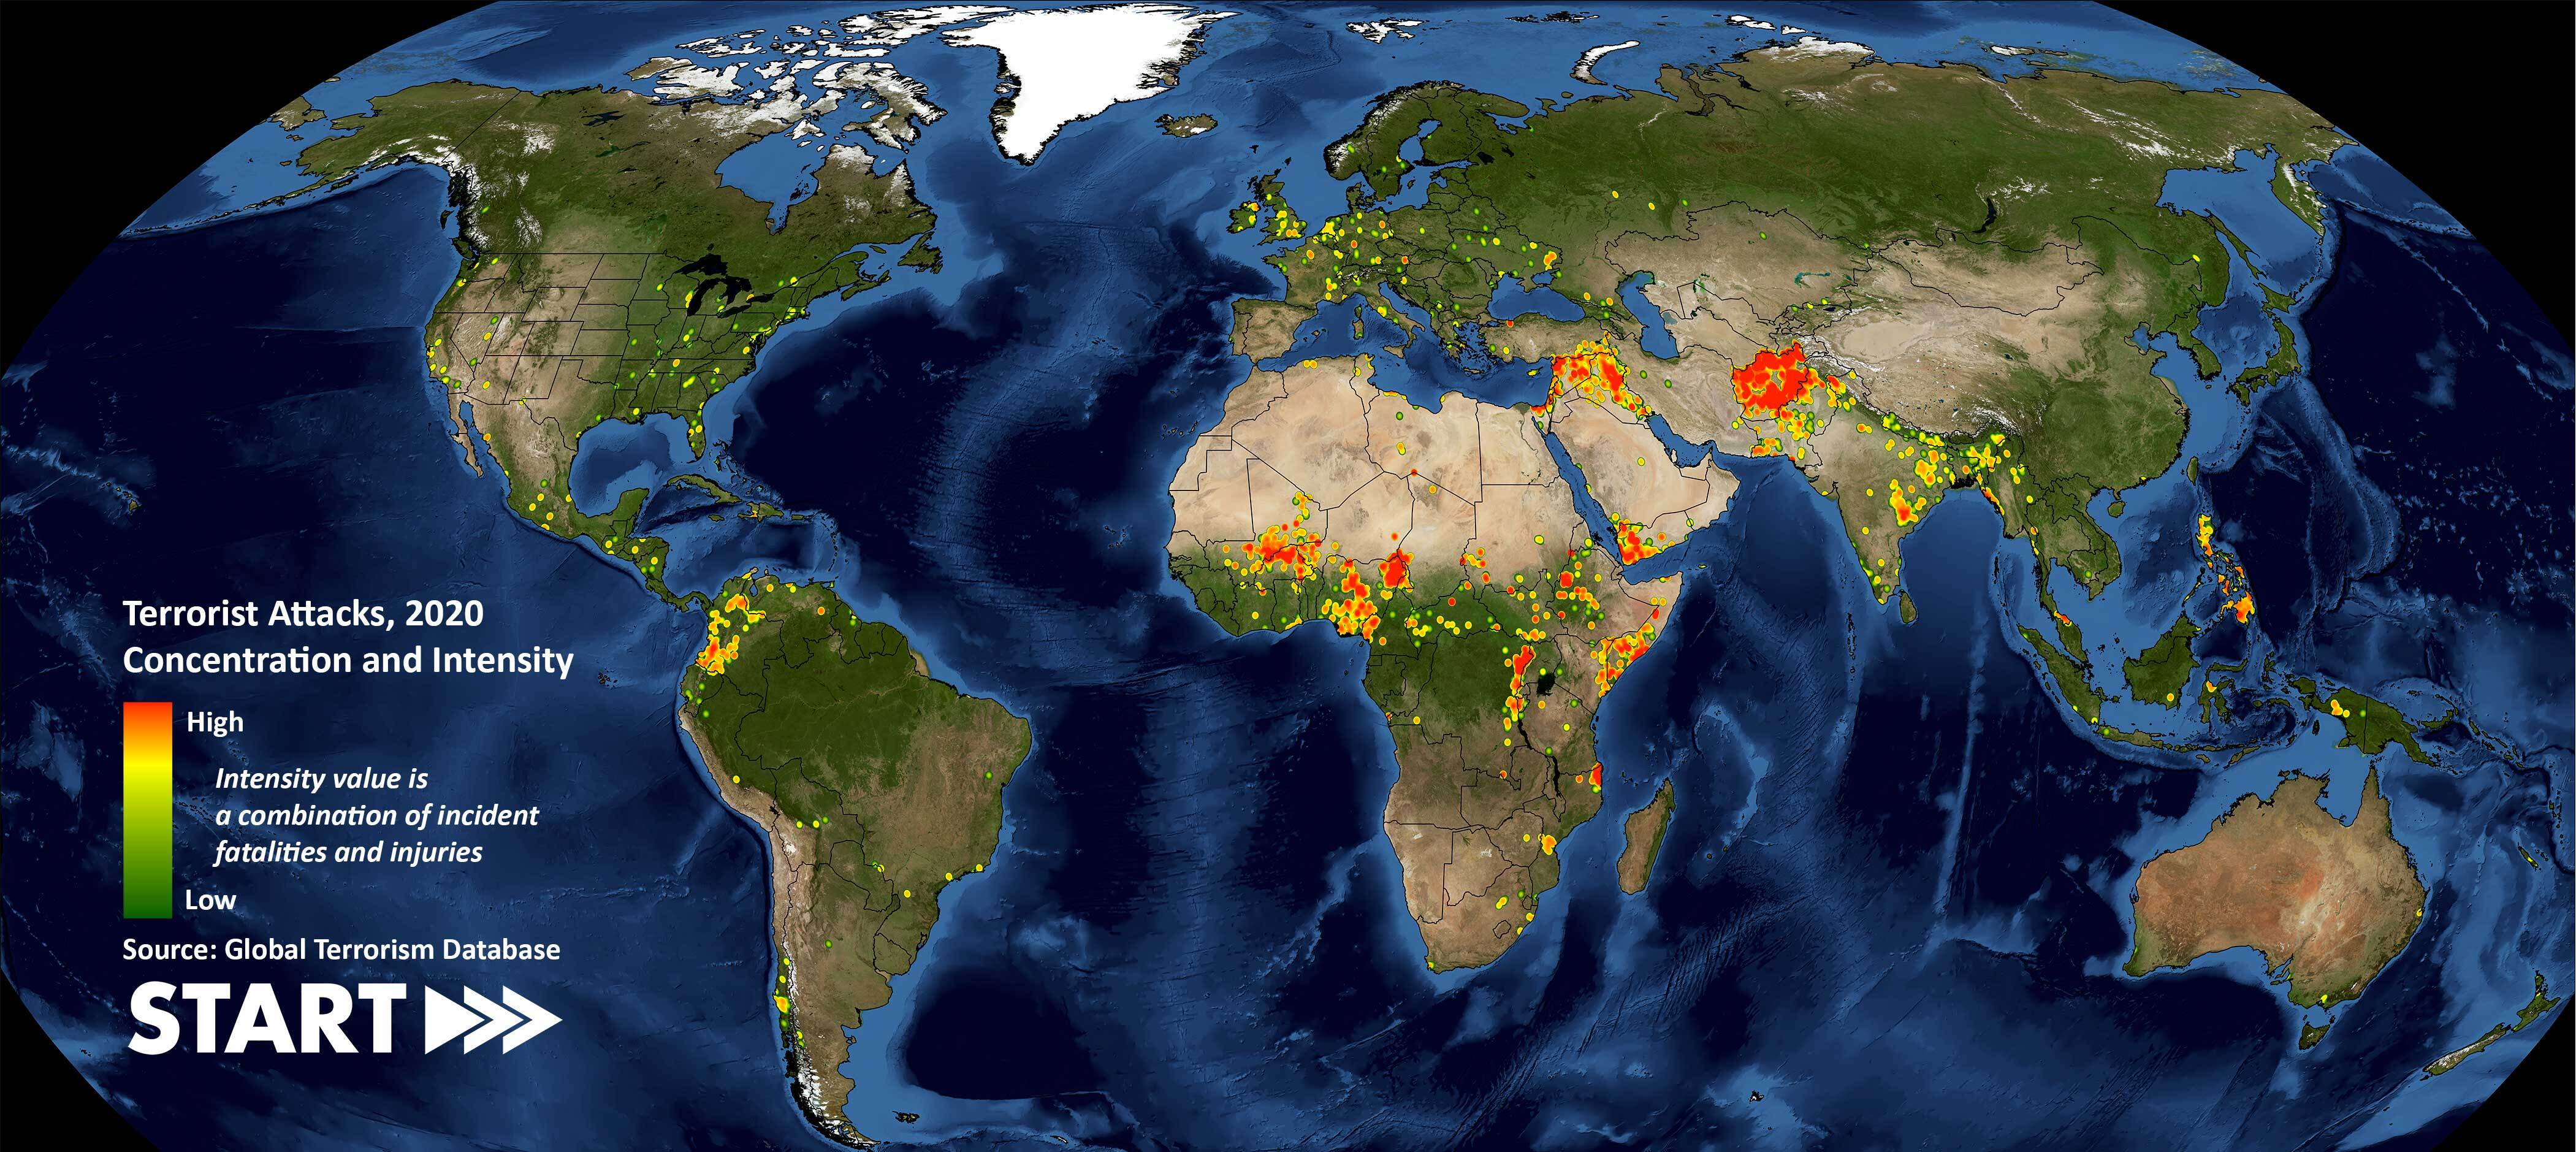
\includegraphics[width=\textwidth,height=\textheight,keepaspectratio]{START_GTD-Heatmap_2020.jpg}
	\end{figure}
\end{frame}


\begin{frame} 
	\frametitle{\LARGE{Terrorism Statistics by Group}}
	\begin{figure}[ht!]
		\centering
		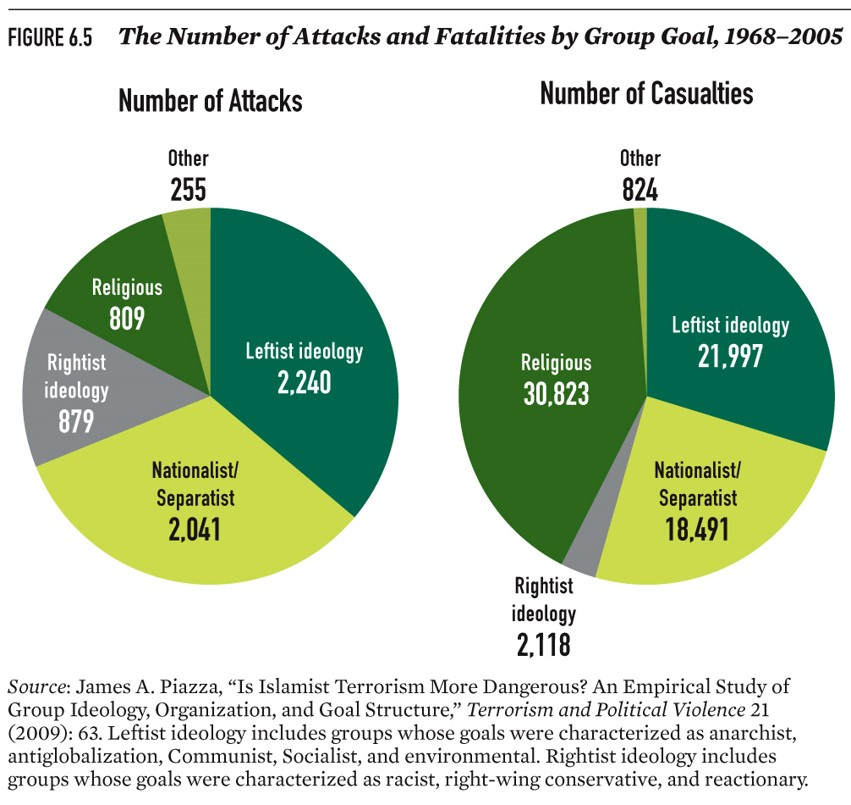
\includegraphics[width=\textwidth,height=\textheight,keepaspectratio]{Piazza2005.jpg}
	\end{figure}
\end{frame}

\begin{frame} 
\frametitle{\LARGE{Transnational Attacks over Time}}
\begin{figure}[ht!]
	\centering
	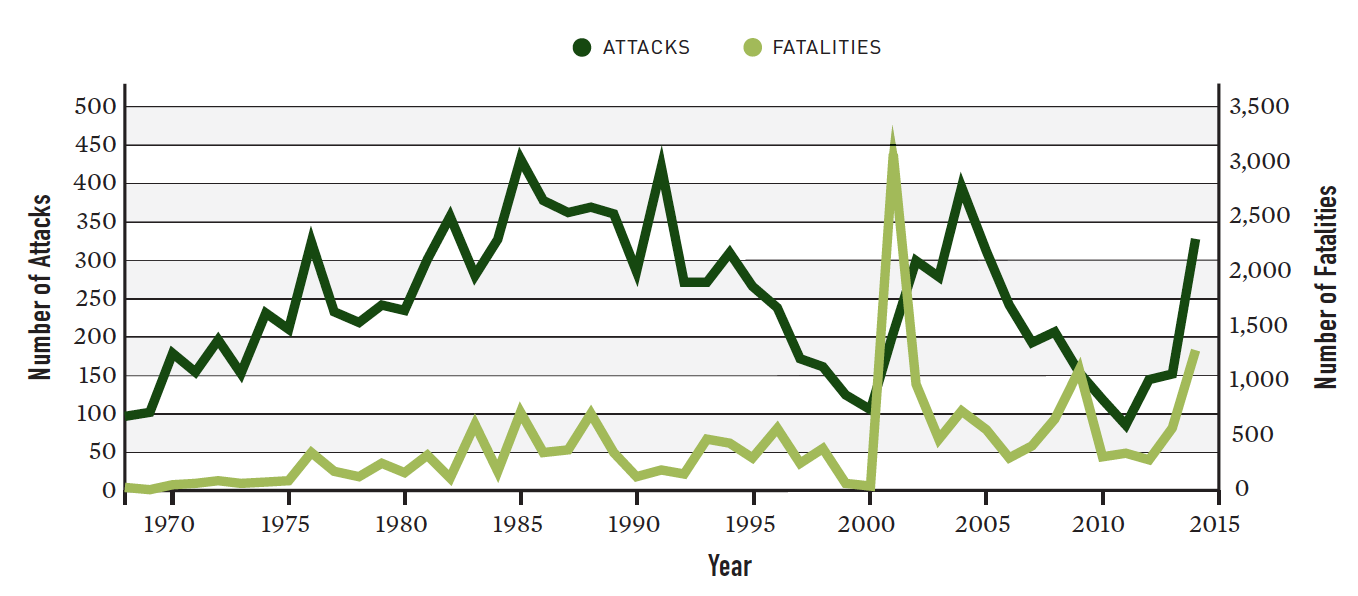
\includegraphics[width=\textwidth,height=0.8\textheight,keepaspectratio]{./trans_attacks.png}
\end{figure}
\end{frame}

\begin{frame} 
	\frametitle{\LARGE{Worldwide Attacks and Fatalities}}
	\begin{figure}[ht!]
		\centering
		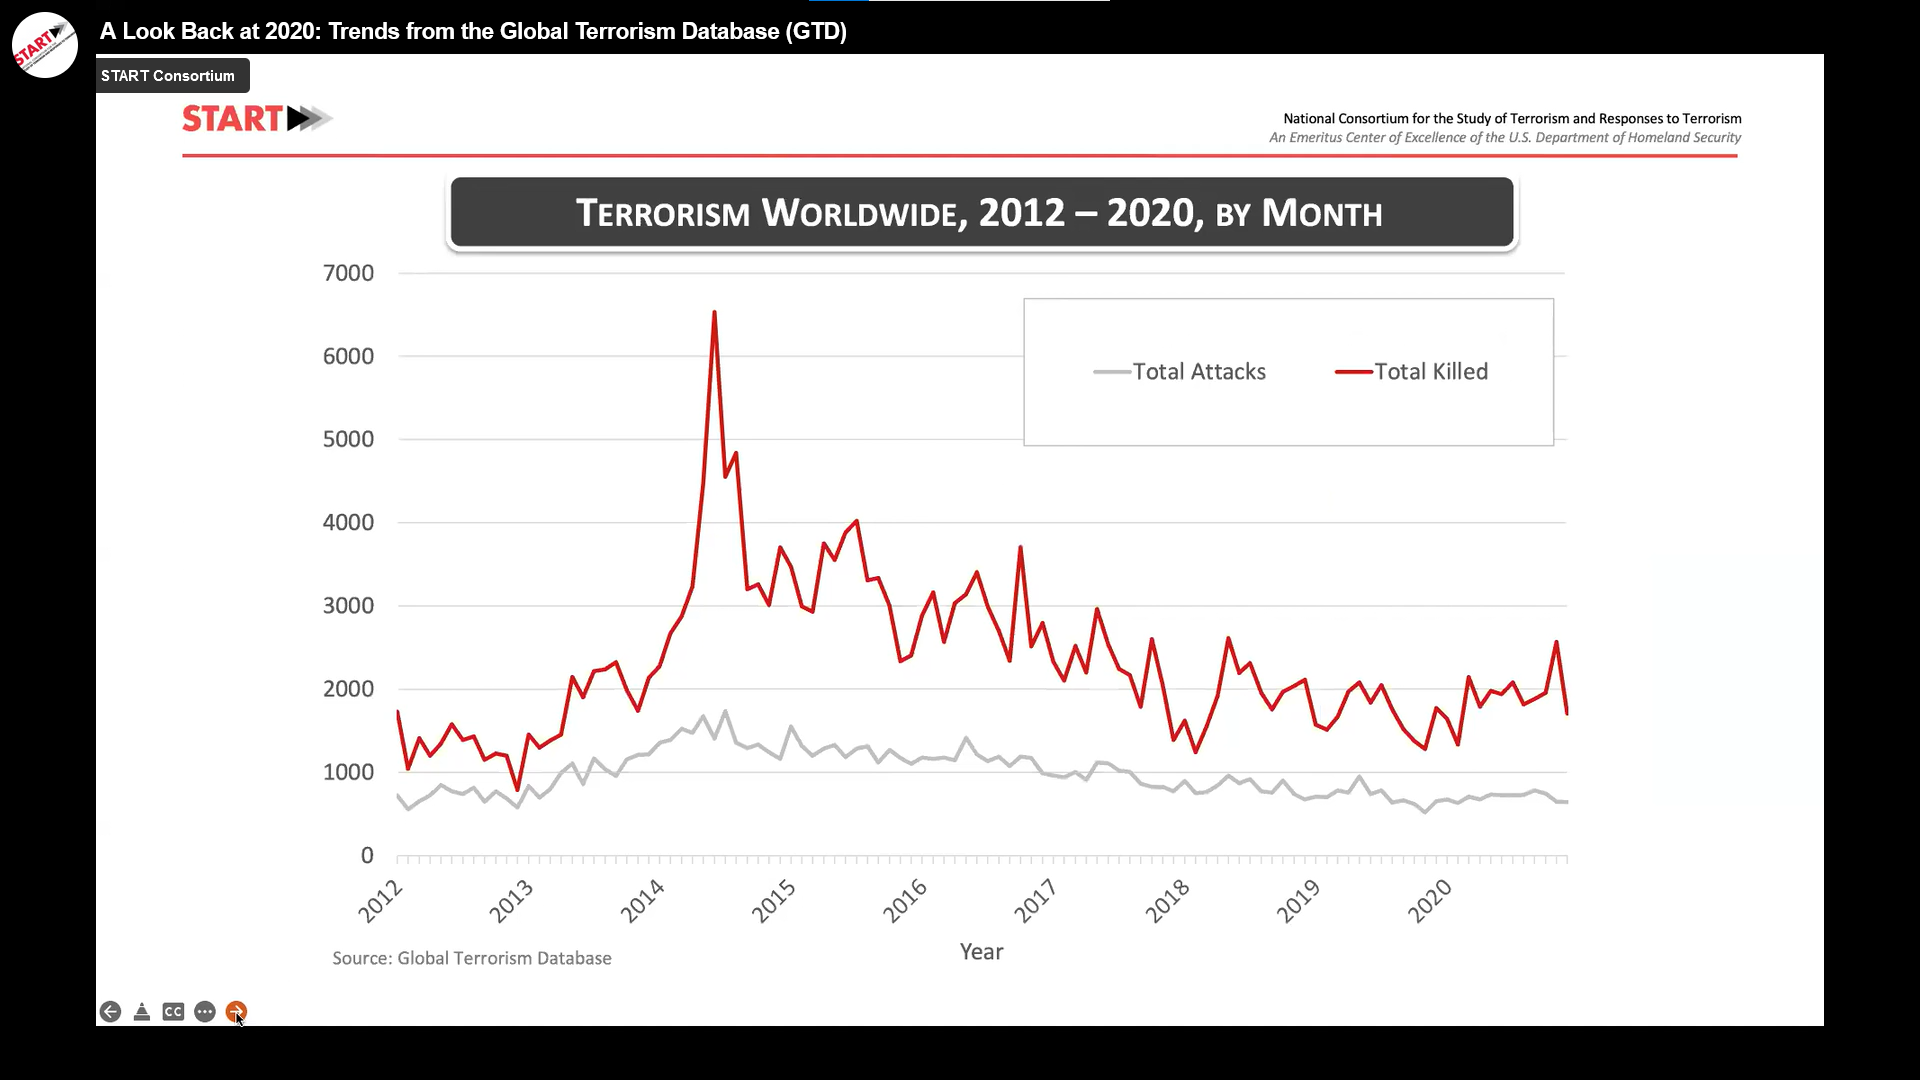
\includegraphics[width=\textwidth,height=\textheight,keepaspectratio]{terrorism2012.png}
	\end{figure}
\end{frame}

\begin{frame} 
	\frametitle{\LARGE{Civil War and Terrorism, 2010-2016}}
	\begin{figure}[ht!]
		\centering
		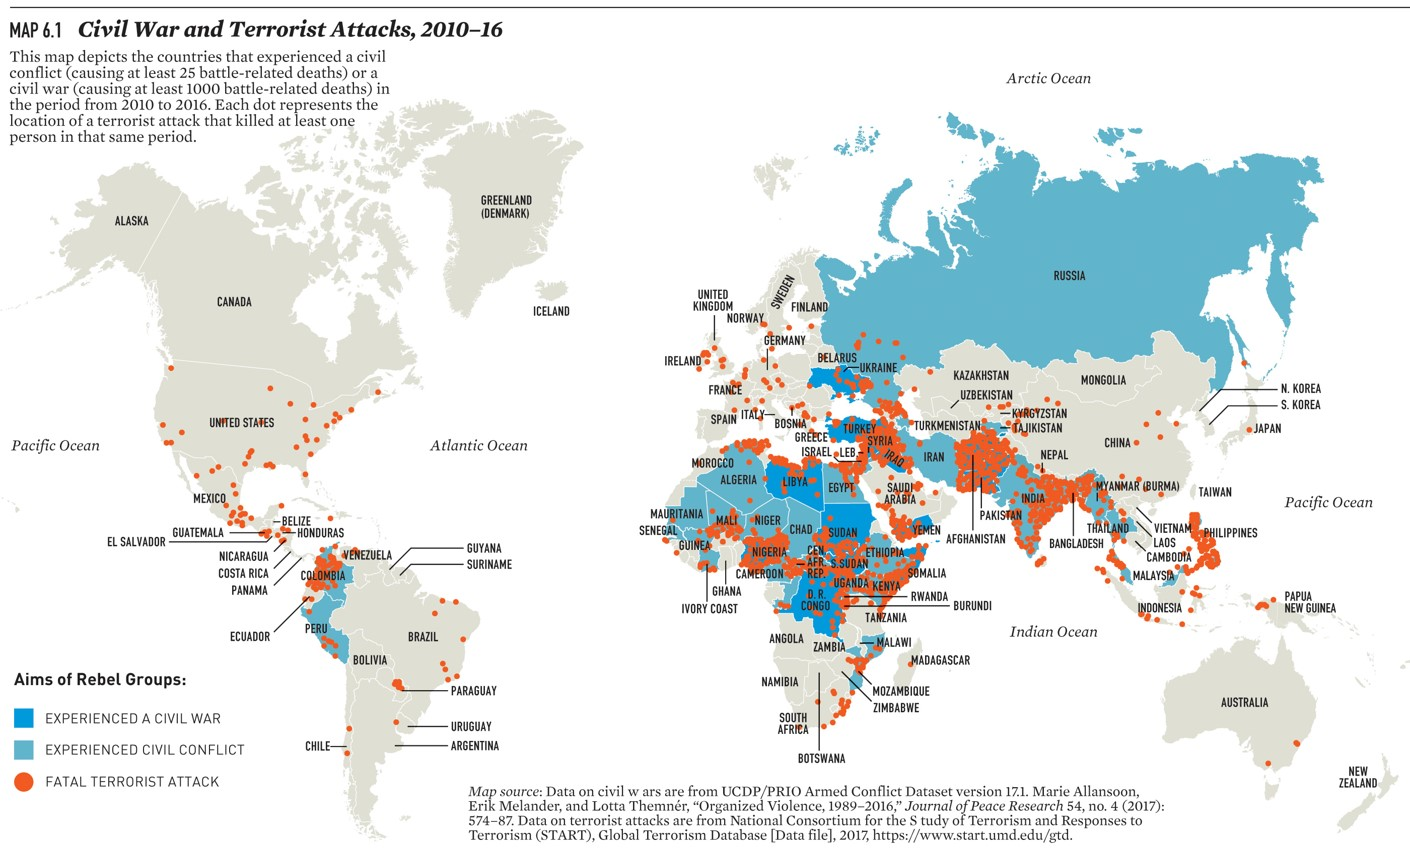
\includegraphics[width=\textwidth,height=0.8\textheight,keepaspectratio]{civwarter.jpg}
	\end{figure}
\end{frame}

\begin{frame} 
	\frametitle{\LARGE{Attacks and Fatalities by State, 2020}}
	\begin{figure}[ht!]
		\centering
		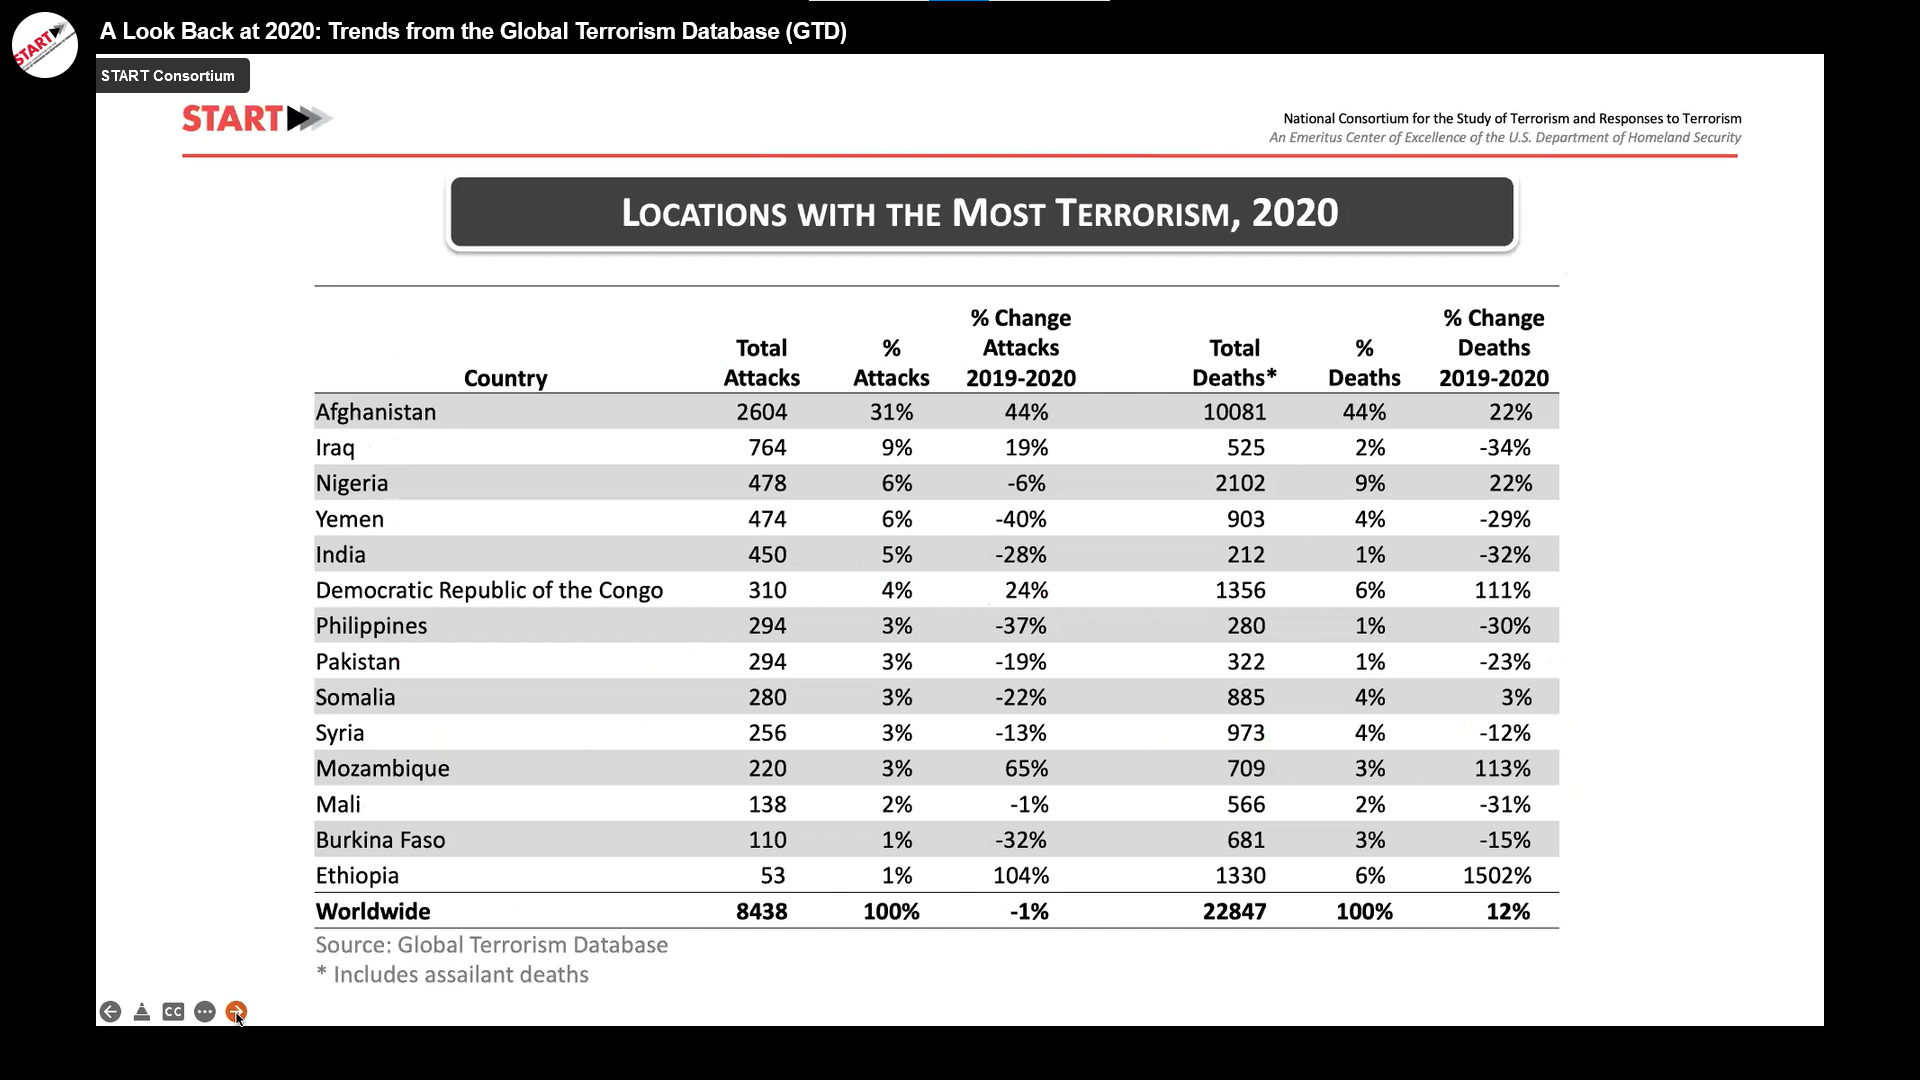
\includegraphics[width=\textwidth,height=\textheight,keepaspectratio]{terrorismlocations2020.png}
	\end{figure}
\end{frame}

\begin{frame} 
	\frametitle{\LARGE{Attacks and Fatalities by Group, 2020}}
	\begin{figure}[ht!]
		\centering
		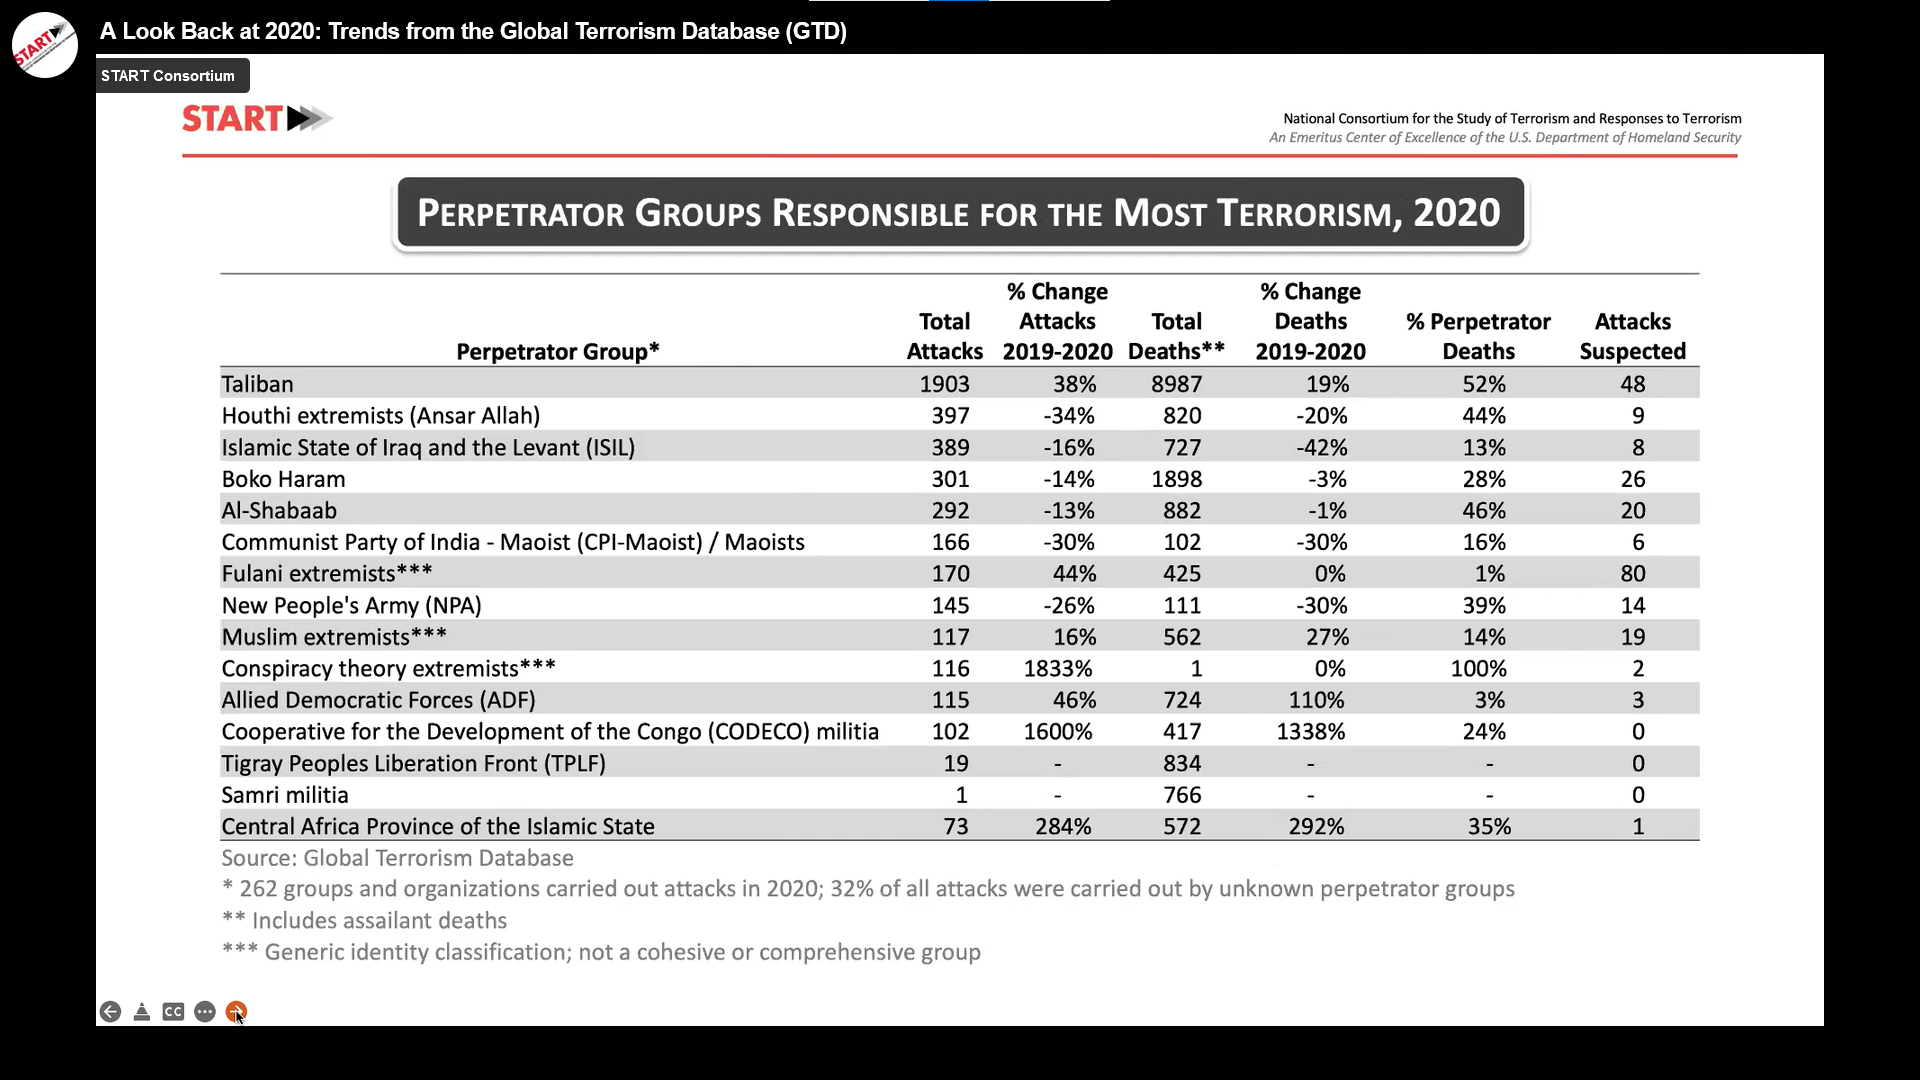
\includegraphics[width=\textwidth,height=\textheight,keepaspectratio]{terrorismperp2020.png}
	\end{figure}
\end{frame}

\begin{frame} 
	\frametitle{\LARGE{Terrorism in the US, 2012-2020}}
	\begin{figure}[ht!]
		\centering
		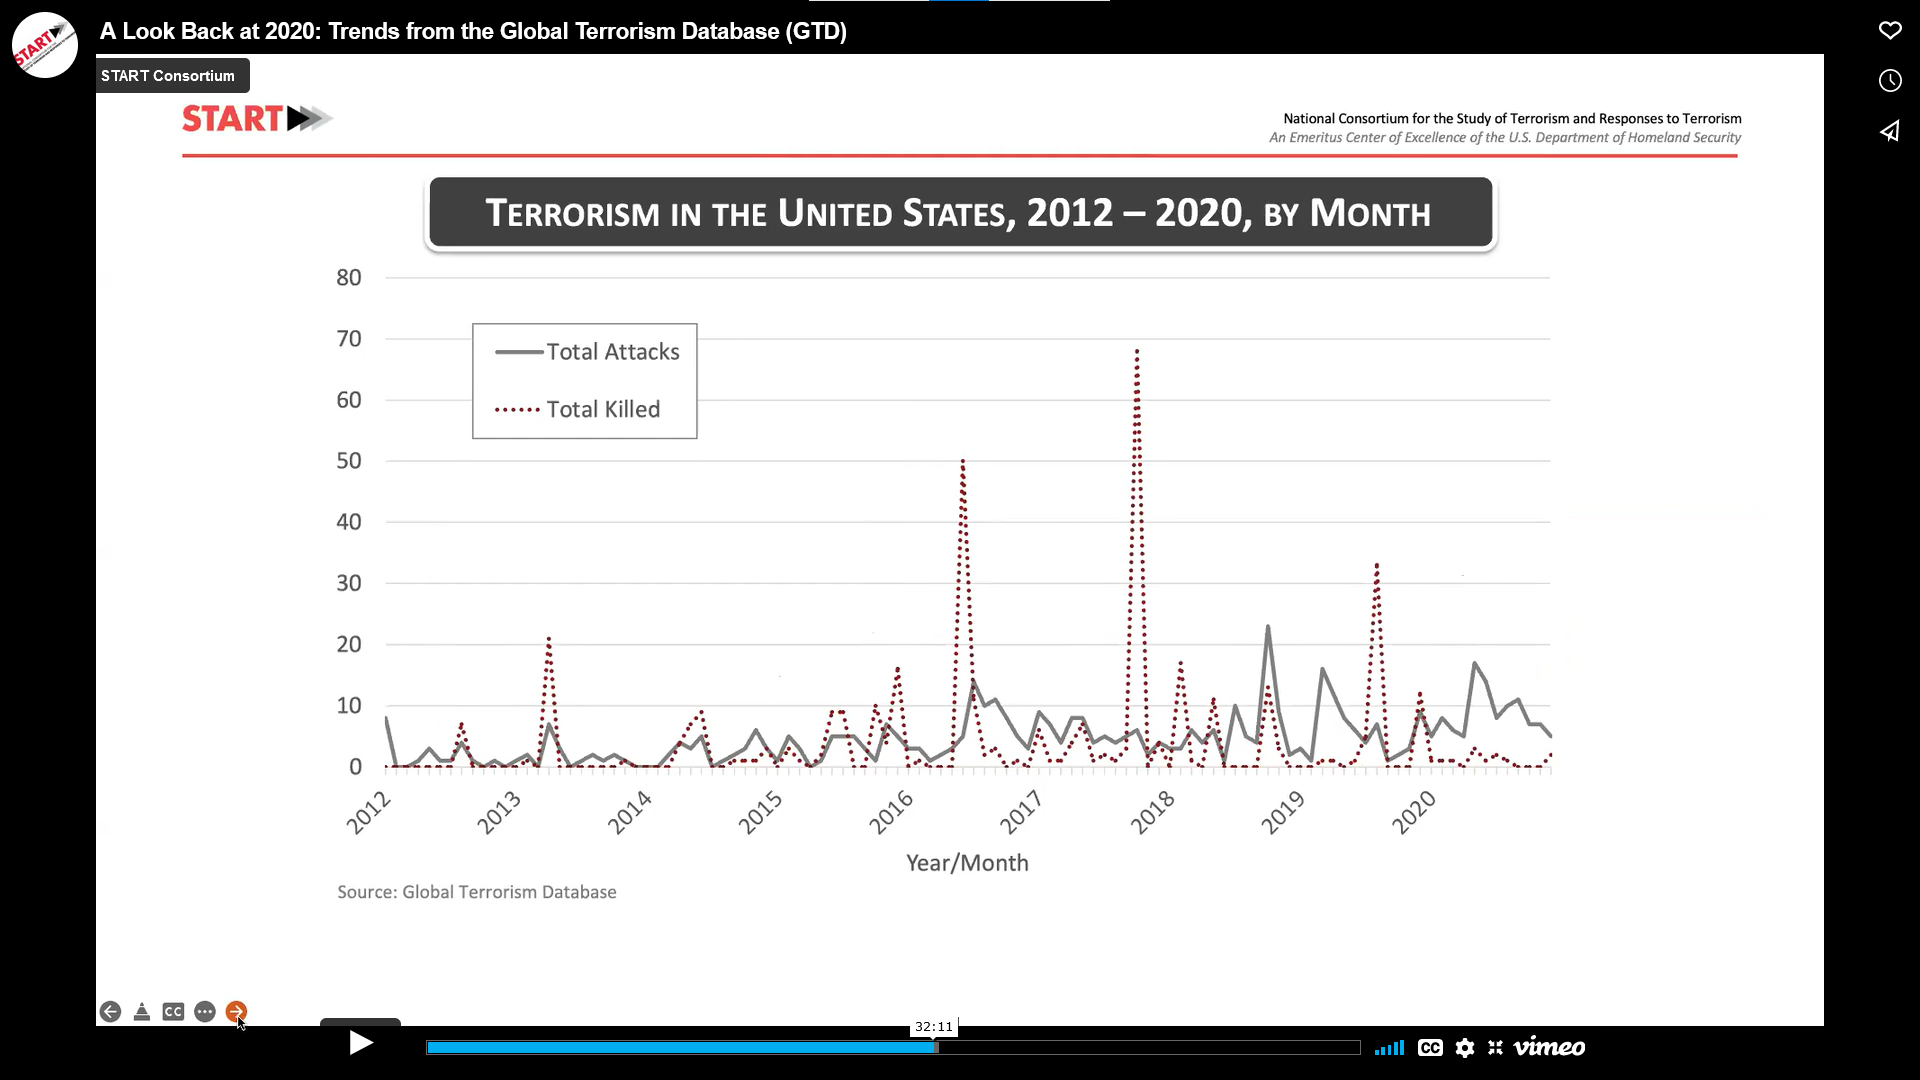
\includegraphics[width=\textwidth,height=\textheight,keepaspectratio]{USterrorism2020.png}
	\end{figure}
\end{frame}

\begin{frame} 
	\frametitle{\LARGE{Perpetrators in US and Europe, 2020}}
	\begin{figure}[ht!]
		\centering
		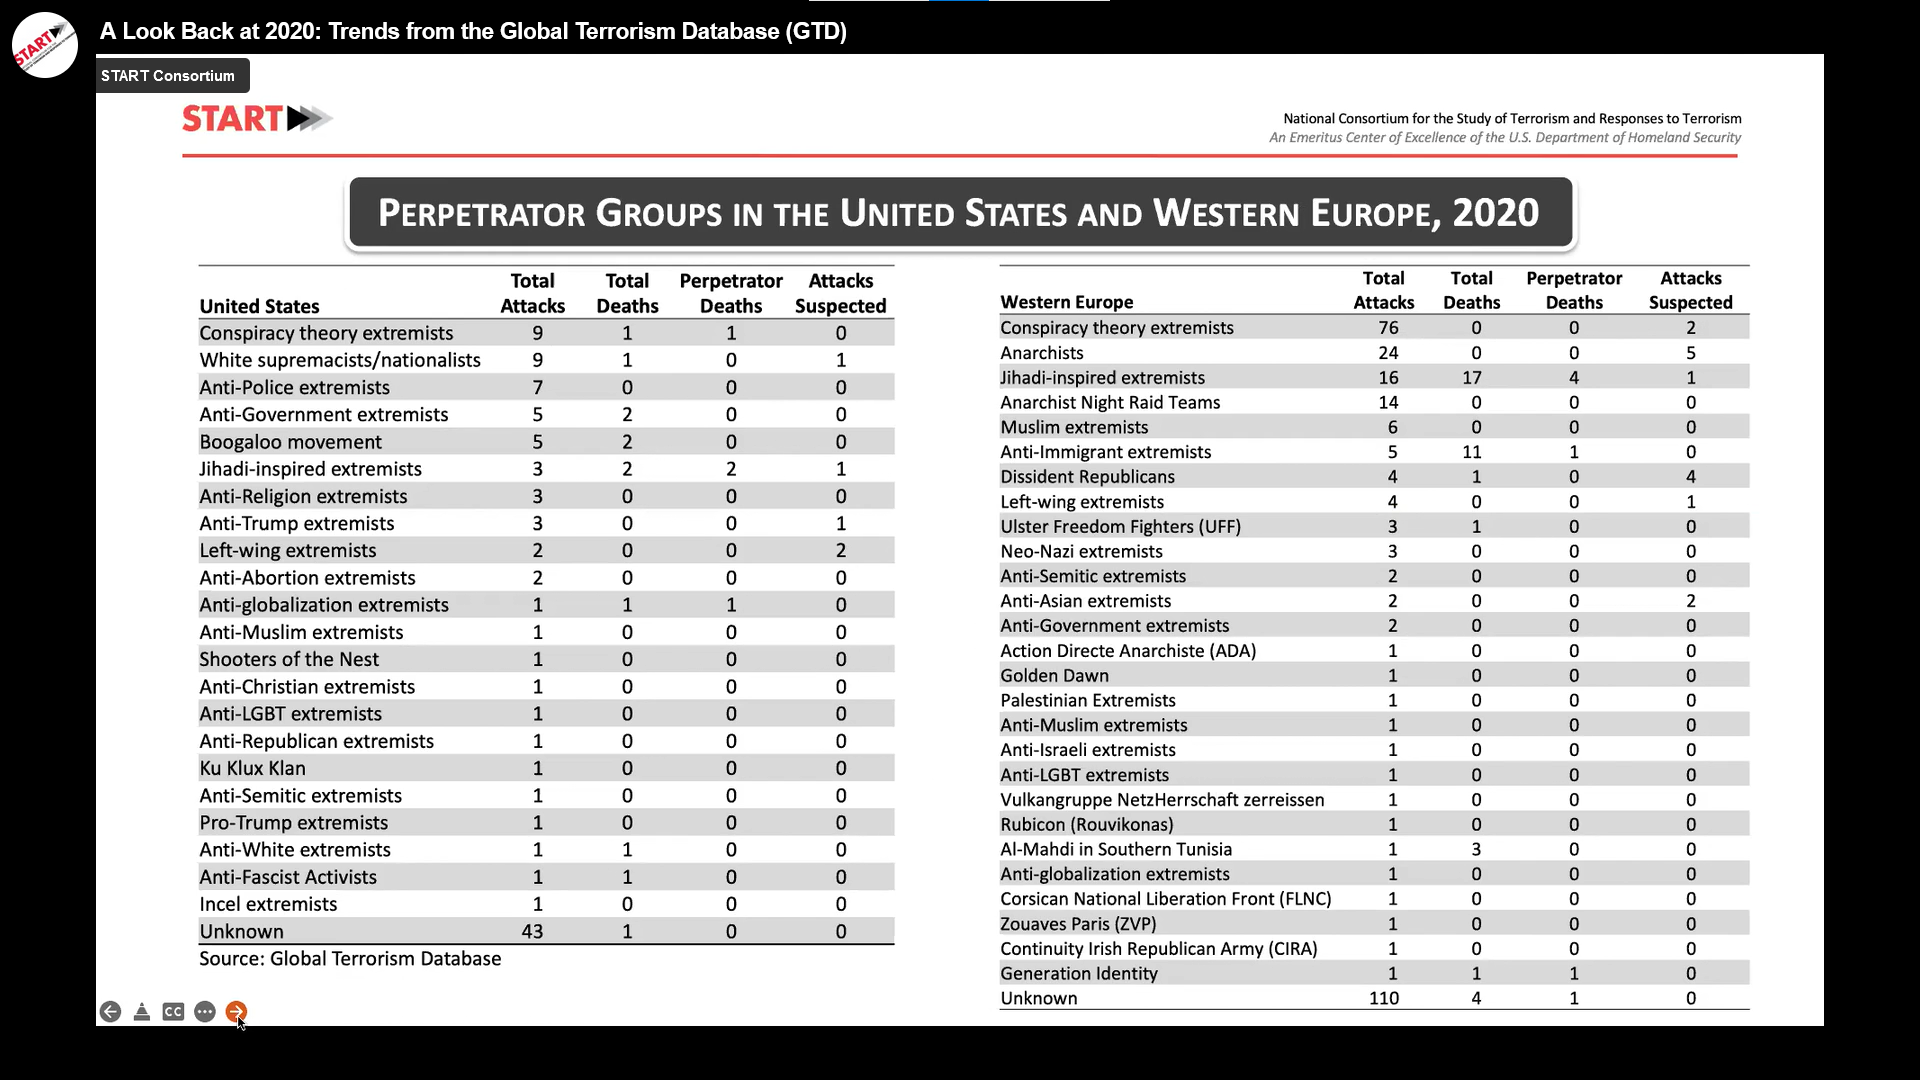
\includegraphics[width=\textwidth,height=\textheight,keepaspectratio]{perpetrators2020.png}
	\end{figure}
\end{frame}

\begin{frame} 
	\frametitle{\LARGE{Terrorism vs. US Car Crashes}}
	\begin{figure}[ht!]
		\centering
		\includegraphics[width=\textwidth,height=.9\textheight,keepaspectratio]{crashes.jpg}
	\end{figure}
\end{frame}

\begin{frame} 
	\frametitle{\LARGE{Terrorism Data Takeaways}}
	From this data, we know that:
	\begin{itemize}
		\item Most terrorism is domestic, not transnational. \pause
		\item Most transnational terrorism is not religious in nature. \pause
		\item Terrorism, especially transnational terrorism, is not solely religiously motivated. \pause
		\item However, religiously motivated terrorism causes disproportionately high casualties compared to other motivations. 
		
	\end{itemize}
\end{frame}

\begin{frame} 
	\frametitle{\LARGE{Terrorism Data Takeaways}}
From this data, we also know that:
	\begin{itemize}
		\item Terrorism and civil war sometimes overlap, but the presence of one does not automatically mean the presence of the other. \pause
		\item In an American context, terrorism is typically not carried out by Islamist extremists. \pause
		\item Deaths from any type of terrorism are disproportionately covered by the media, leading to inaccurate risk perceptions (\href{https://ourworldindata.org/terrorism}{further reading}). \pause
		\item \textbf{You should not be worried about dying of terrorism in your daily life.}
		
	\end{itemize}
\end{frame}

\begin{frame} 
\frametitle{\LARGE{The Rationality of Terrorism}}
\begin{itemize}
	    \item Public discourse routinely suggests that terrorists are bloodthirsty, crazed fanatics. \pause 
	    \item Terrorism is a deliberately chosen \textit{strategy}, which raises a question: is its use rational? \pause
		\item Rational actors pick strategies that maximize their chances of getting the outcome they want. \pause 
		\item To determine whether terrorism is rational, we must determine why groups use it.
\end{itemize}
\end{frame}

\begin{frame} 
	\frametitle{\LARGE{The Rationality of Terrorism}}
	\begin{itemize}
		\item \textbf{The end goal of a strategy of terrorism is to extract concessions from an adversary, not by defeating them, but by inflicting costs on their civilians such that the state gives concessions to prevent those costs.} \pause
		\item Why choose terrorism over other strategies, such as participation in legitimate political processes or insurgency? \pause
		\item Because actors using terrorism are generally weak in two ways...
	\end{itemize}
\end{frame}


\begin{frame} 
\frametitle{\LARGE{Weakness 1: Capabilities}}
Terrorist actors have very weak capabilities. \pause
\begin{itemize}
		\item Nonstate actors can rarely match the strength of the state. \pause 
		\item If these actors can mobilize sufficient strength, they can engage in insurgency. \pause 
		\item Terrorist groups are generally even smaller and weaker than the insurgent groups that start civil wars.
\end{itemize}
\end{frame}

\begin{frame} 
\frametitle{\LARGE{Weakness 2: Demands and Extremism}}
Terrorist groups are weak relative to the magnitude of their demands.
\begin{itemize}
		\item Groups using terrorism frequently make demands far beyond their power to reasonably achieve. \pause 
		\item Terrorist groups are also comprised of \textbf{extremists}, meaning that their goals and strategies for achieving them are not usually widely shared. \pause 
		\item This extremism limits both the size of their recruitment pool and their ability to engage in the political process. \pause
		\begin{itemize}
			\item Extremists cannot develop a broad enough base of support to engage in insurgency, much less in legitimate political competition. \pause
			\item Some extremist viewpoints are also excluded from the political process by design.
		\end{itemize} 
\end{itemize}
\end{frame}

\begin{frame} 
	\frametitle{\LARGE{A Weapon of the Weak}}
	\begin{itemize}
		\item Extremist ideology has only limited appeal, and as such extremists are: 
		\begin{itemize}
			\item Unable to gain support for meaningful legitimate political participation. \pause
			\item Unable to generate enough popular support to mobilize for civil war or direct violent confrontation to achieve their goals. \pause
		\end{itemize}
	\item Given these limitations, \textbf{terrorism is a weapon of the weak, used to try to extract concessions from the target government.}
	\item Thus, \textbf{the use of terrorism is rational for such weak actors.}		
	\end{itemize}
\end{frame}

\begin{frame} 
	\frametitle{\LARGE{How Does Terrorism Work?}}
Terrorism requires two elements: shock and randomness.
	\begin{itemize}
		\item \textbf{Shock}: terrorist violence is sensational and notable for its methods. For example...		
	\end{itemize}
\end{frame}

\begin{frame} 
	\frametitle{\LARGE{ISIS Executions}}
	\begin{figure}[ht!]
		\centering
		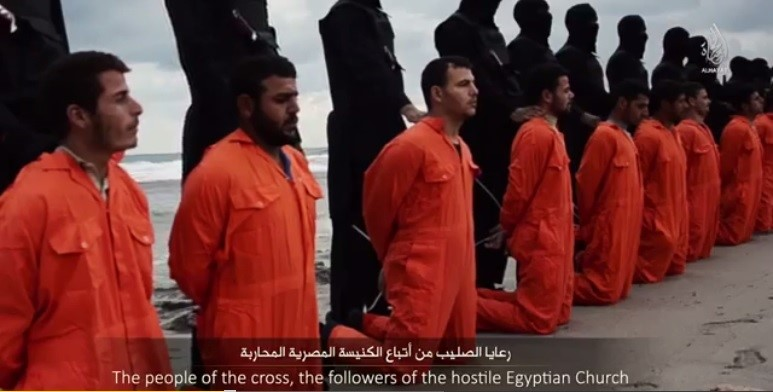
\includegraphics[width=\textwidth,height=0.9\textheight,keepaspectratio]{ISISexec.jpg}
	\end{figure}
\end{frame}

\begin{frame} 
	\frametitle{\LARGE{How Does Terrorism Work?}}
	Terrorism requires two elements: shock and randomness.
	\begin{itemize}
		\item \textbf{Shock}: terrorist violence is sensational and notable for its methods. For example...	
		\item Terrorist violence tends to take forms that are not seen in ``legitimate" warfare: suicide bombings, vehicles as improvised weapons, gruesome executions, etc. \pause
		\item The goal here is a heightened, visceral emotional response.	
	\end{itemize}
This emotional response is paired with...
\end{frame}

\begin{frame} 
	\frametitle{\LARGE{How Does Terrorism Work?}}
Terrorism requires two elements: shock and randomness.
	\begin{itemize}
		\item \textbf{Randomness}: terrorist attacks occur unpredictably, seemingly at random, frequently in crowded places where they interrupt everyday life of civilians. \pause
		\item \textbf{The goal of any given attack is not to harm those \textit{specific} civilians who were hurt, but to create fear in the broader population that the random nature of the attacks means they could be next.} \pause
		\item This is further heightened by the visceral emotional response created by these attacks.
	\end{itemize}
\end{frame}

\begin{frame} 
	\frametitle{\LARGE{How Does Terrorism Work?}}
	\begin{itemize}
		\item Recall the definition of terrorism: committed ``for the purpose of influencing a group larger than the immediate victims." \pause
		\item The whole point of an attack is to spread fear throughout broader society, \textbf{even though from a statistical viewpoint almost all citizens have nothing to fear.}
		\item The overarching goal of a terrorist group is to extract concessions from its target government, and this violence can (in theory) cause citizens to pressure their government to stop the terrorism - even if it involves making concessions.
	\end{itemize}
\end{frame}

\begin{frame} 
\frametitle{\LARGE{Terrorism and Bargaining Failure}}
\begin{itemize}
		\item Why don't states and terrorist groups bargain? \pause
		\item While terrorism's costs may be lower than those of a conventional war or insurgency, they are still costs. \pause
		\item If we expand our definition of costs to include psychological damage and the stress of constant fear on the general population, terrorism has sufficient costs that we would expect some kind of bargaining. 
\end{itemize}
\end{frame}

\begin{frame} 
\frametitle{\LARGE{Terrorism and Incomplete Information}}
Incomplete information problems are endemic for terrorist groups:
\begin{itemize}
		\item Terrorist groups are clandestine by nature, making them unable to show their strength without being exposed to capture by the state. \pause
		\item Terrorist groups have substantial incentives to misrepresent strength, and the state knows this. \pause
		\item Actually carrying out attacks may be the only way for a group to credibly signal its capabilities and resolve.
\end{itemize}
\end{frame}

\begin{frame} 
	\frametitle{\LARGE{Terrorism and Commitment Problems}}
Commitment problems are similar to those facing rebels:
	\begin{itemize}
		\item As with disarming rebels, terrorists struggle to get a credible commitment that the state will not retaliate after they demobilize and reveal themselves. \pause
		\item Fragmented terrorist groups may have leaders willing to honor a deal, but those leaders may be unable to prevent cells from engaging in attacks. \pause
		\item Additionally, the state also knows that leaders have incentives to misrepresent their level of control. 
	\end{itemize}
\end{frame}

\begin{frame} 
	\frametitle{\LARGE{Terrorism and Indivisibility Problems}}
Indivisibility problems may also occur:
	\begin{itemize}
		\item Terrorist extremist views may shrink the bargaining range. \pause
		\item Terrorist ideology may lead them to make all-or-nothing indivisible demands.
	\end{itemize}
\end{frame}

\begin{frame} 
	\frametitle{\LARGE{Terrorist Strategies of Violence}}
	\begin{itemize}
		\item \textbf{The end goal of a strategy of terrorism is to extract concessions from an adversary, not by defeating them, but by inflicting costs on their civilians such that the state gives concessions to prevent those costs.} \pause
		\item This implies the existence of multiple ``audiences" for any given act of terrorism:
		\begin{enumerate}
			\item Government of the target state.
			\item Population of the target state.
			\item The terrorist group's claimed constituency (``home population"). \pause
		\end{enumerate}
	\item This means that terrorism as a strategy can also be used for multiple different tactical aims.
	\end{itemize}
\end{frame}

\begin{frame} 
	\frametitle{\LARGE{Tactics of Terrorism}}
	\begin{enumerate}
		\item \textbf{Coercion}
		
		\item \textbf{Provocation}
		
		\item \textbf{Spoiling} 
		
		\item \textbf{Outbidding}
	\end{enumerate}
\end{frame}

\begin{frame} 
\frametitle{\LARGE{Tactics of Terrorism: Coercion}}
\begin{itemize}
		\item \textbf{Coercion}: encourage policy change by engaging in violence and threatening future violence (implicitly or explicitly). \pause 
		\item Here, the attack itself is a form of costly signaling of terrorist resolve and capability. \pause
		\item To be successful, target must care about these costs in some way: \pause
		\begin{itemize}
			\item Domestic politics favor negotiation (ex: doves vs. hawks). \pause
			\item Public perceptions of threat levels are (irrationally) high. \pause
			\item State has responded favorably (from terrorist POV) to prior attacks.
		\end{itemize}

		
\end{itemize}
\end{frame}

\begin{frame} 
	\frametitle{\LARGE{Tactics of Terrorism: Provocation}}
	\begin{itemize}
		\item \textbf{Provocation}: induce government into indiscriminate violence that pushes individuals to join or be sympathetic toward terrorist group's cause. \pause
		\item To be successful, this requires the terrorist group's claimed constituency to be uncertain about the target's true intentions towards them. \pause
		\item If terrorists provoke indiscriminate reprisal violence, this will confirm the worst suspicions of their constituency.
		\item Ex: most US drone strikes?
	\end{itemize}
\end{frame}

\begin{frame} 
	\frametitle{\LARGE{Tactics of Terrorism: Spoiling}}
	\begin{itemize}
		\item \textbf{Spoiling}: sabotaging a possible peace deal between a moderate group within a terrorist faction (and/or its claimed constituency) and the target state's government. \pause 
		
		\item To be successful, this must convince the target government that moderates cannot or will not prevent their extremists from engaging in future attacks. \pause
		\item This sabotages the credibility of any deal.
		\item Ex: failure of Oslo Accords between Israel and Palestine.
	\end{itemize}
\end{frame}

\begin{frame} 
	\frametitle{\LARGE{Tactics of Terrorism: Outbidding}}
	\begin{itemize}
		\item \textbf{Outbidding}: occurs when two or more terrorist groups devoted to the same cause, attempting to draw on the same support base, use attacks to signal their superiority. \pause
		\item Attacks help groups to signal their extreme views relative to each other. Their hope is that the support base views more extreme groups as more effective ones.
		\item Ex: Fatah vs. Hamas in Palestine
		
	\end{itemize}
\end{frame}




\begin{frame} 
\frametitle{\LARGE{Does Terrorism Work?}}
\begin{itemize}
		\item Substantial debate following 9/11 about whether terrorism is effective. \pause 
		\item Much of the debate about whether or not terrorism works boils down to how we define \emph{success} for a group. \pause 
		\item Even so, the numbers do not look good...
\end{itemize}
\end{frame}

\begin{frame} 
	\frametitle{\LARGE{Terrorism Success Rates}}
	\begin{figure}[ht!]
		\centering
		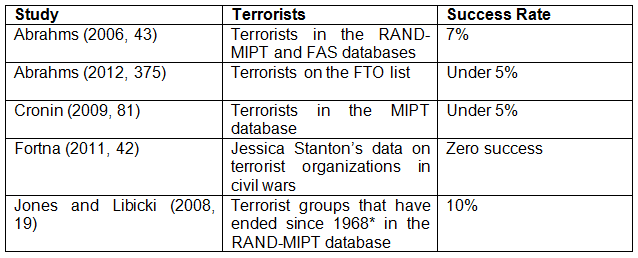
\includegraphics[width=\textwidth,height=0.9\textheight,keepaspectratio]{terrorsuccess.png}
	\end{figure}
\end{frame}

\begin{frame} 
	\frametitle{\LARGE{Does Terrorism Work?}}
	\begin{itemize}
		\item Approximately 90\% of terrorist groups collapse within 4-6 years of formation, as the state eliminates them or they fragment into splinter groups. \pause
		\item Terrorist groups generally fail to accomplish their stated objectives before collapsing. \pause
		\item In those rare cases of success, the group must survive and make attacks for so long that it can convince the state that it must be negotiated with (ex: Taliban circa early 2020). \pause
		\item In rare instances the terrorist groups can extract concessions, but they generally fail to do so. \pause
		\begin{itemize}
			\item States may respond by hardening their positions; strikes may provoke a rally effect.
		\end{itemize}
	\end{itemize}
\end{frame}

\begin{frame} 
\frametitle{\LARGE{What About Terrorism and Civil Wars?}}
Earlier slides show a substantial geographical overlap of terrorism and civil wars.
\begin{itemize}
		\item Fortna (2014) looks at the difference in outcome of rebel groups that use or do not use terrorist tactics. \pause 
		\item She finds that nonterrorist rebel groups are more successful. \pause 
		\item However, wars last longer when rebels use terrorist tactics. \pause 
		\item Rebels face a dilemma: terrorism might help a group survive, but will not help it to achieve its broader goals. 
\end{itemize}
\end{frame}

\begin{frame} 
\frametitle{\LARGE{Terrorist Rebels in Civil Wars}}
\begin{figure}[ht!]
	\centering
	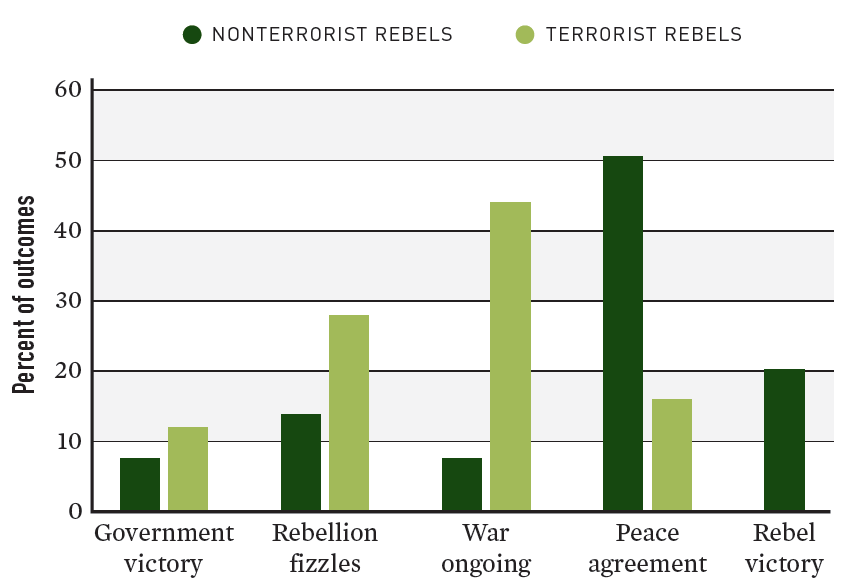
\includegraphics[width=\textwidth,height=0.8\textheight,keepaspectratio]{./terr_success.png}
\end{figure}
\end{frame}

\begin{frame} 
	\frametitle{\LARGE{What About Terrorism and Civil Wars?}}
Notably, one path to survival for terrorist groups is to transition into an insurgency.
	\begin{itemize}
		\item If a terrorist group can manage to become an insurgency, they may be more likely to succeed. \pause
		\item Terrorist groups and insurgent groups both have low success rates, but those of terrorist groups are even lower than those of rebel groups. 
	\end{itemize}
\end{frame}

\begin{frame} 
	\frametitle{\LARGE{Counter-Terrorism Strategies}}
	States facing terrorism have several of options.
	\begin{enumerate}
		\item \textbf{Deterrence}
		\item \textbf{Preemption}
		\item \textbf{Defensive measures}
		\item \textbf{Criminalization} 
		\item \textbf{Negotiation}
	\end{enumerate}
\end{frame}

\begin{frame} 
\frametitle{\LARGE{Counter-Terrorism Strategy: Deterrence}}
\begin{itemize}
		\item \textbf{Deterrence}: threaten massive retaliation for any given terrorist incident. \pause
		\item If asked, most states would describe this as their default stance. \pause
		\item To be successful, the state must be able to strike back with devastating force, in an accurate manner.
		\item Drawbacks and limitations: \pause
		\begin{itemize}
			\item Lack of credibility will hinder effectiveness. \pause
			\item Even when successful, it risks playing into a terrorism strategy of provocation.
		\end{itemize}
\end{itemize}
\end{frame}

\begin{frame} 
	\frametitle{\LARGE{Counter-Terrorism Strategy: Preemption}}
	\begin{itemize}
		\item \textbf{Preemption}: eliminate terrorist groups before they can strike (again). \pause 
		\item A primary strategy of the American War on Terror.
		\item Prerequisite: very high state capacity. \pause
		\item Drawback is a very high cost in terms of material, committed state security forces, intelligence-gathering efforts, etc.  
	\end{itemize}
\end{frame}

\begin{frame} 
	\frametitle{\LARGE{Counter-Terrorism Strategy: Defensive Measures}}
	\begin{itemize} 
		\item \textbf{Defensive measures}: visibly raise the costs of executing attacks on a given target. \pause
		\item Frequently involves making potential targets harder to infiltrate or harder to damage.
		\item Examples: intended purpose of TSA screening, bollards beside roads.
		\item Drawbacks:
		\begin{itemize}
			\item Also costly (installing physical measures, training and paying staff) \pause
			\item As these measures are visible by definition, they may just shift attacks towards less-defended targets. 
		\end{itemize}
	\end{itemize}
\end{frame}

\begin{frame} 
	\frametitle{\LARGE{Counter-Terrorism Strategy: Criminalization}}
	\begin{itemize}
		\item \textbf{Criminalization}: reactive measure that requires strong international cooperation. Ensure terrorists lack safe haven states and that they will be extradited to face legal penalties for their actions. \pause 
		\begin{itemize}
			\item Successful against airline hijackings in the 1970s. \pause
		\end{itemize}
		\item Drawbacks:
		\begin{itemize}
			\item Requires strong international cooperation. \pause
			\item \textbf{Does not appear to meaningfully impact extremist group decisions.} 
		\end{itemize}
	\end{itemize}
\end{frame}

\begin{frame} 
	\frametitle{\LARGE{Counter-Terrorism Strategy: Negotiation}}
	\begin{itemize}
		\item \textbf{Negotiation}: state attempts to negotiate with the group to secure an end to the violence.
		\item Frequently a de facto last resort. \pause
		\item Sometimes not even considered as a legitimate option. Ex: ``we do not negotiate with terrorists" as a cornerstone of US and UK foreign policy.
		\item Drawbacks:
		\begin{itemize}
			\item Like all negotiation, bargaining failure is possible and made more likely by information and commitment problems. \pause
			\item Inflexibility may lead to needless deaths, especially when other Western states frequently do negotiate with terrorists (\href{https://www.chathamhouse.org/2022/01/we-do-not-negotiate-terrorists-why}{further reading}).
		\end{itemize}
			
	\end{itemize}
\end{frame}

\begin{frame} 
\frametitle{\LARGE{Preemption and the War on Terror}}
\begin{itemize}
	\item Preemption strategies are the defining characteristic of America's War on Terror. \pause
	\item America's declaration of a global War on Terror, following 9/11, was essentially a commitment to a global strategy of preemption by claiming the authority to strike at terrorist targets anywhere on the planet.	
\end{itemize}
\end{frame}

\begin{frame} 
	\frametitle{\LARGE{Preemption Strategies of the US}}
This preemption strategy has involved several elements:
	\begin{itemize}
		\item Extensive use of special forces (most famously to kill Bin Laden). \pause	
		\item Frequent use of detention, often indefinitely, without due process or oversight (e.g. Guantanamo Bay detainees and CIA black site program). \pause
		\item Frequent use of torture (ex: waterboarding). \pause
		\item Extensive use of drone strikes: remotely operated aircraft equipped with missiles.
	\end{itemize}
\end{frame}

%image from https://tek2day.com/2021/06/04/military-applications-will-drive-aws-azure-and-google-cloud-growth-for-decades/
\begin{frame} 
	\frametitle{\LARGE{Drone Strikes}}
	\begin{figure}[ht!]
		\centering
		\includegraphics[width=\textwidth,height=\textheight,keepaspectratio]{drone.png}
	\end{figure}
\end{frame}

\begin{frame} 
	\frametitle{\LARGE{Drone Strikes as Preemption}}
	\begin{itemize}
		\item The US used drone strikes extensively in Afghanistan and Pakistan, as well as Yemen and Somalia. \pause
		\begin{itemize}
			\item Note that the US was only formally at war in one of these states. \pause
		\end{itemize}
		\item The stated rationale was that these were precisely targeted, selective strikes against known terrorists conducted with zero risk to US military personnel. \pause
		\item In Pakistan alone (all data from \href{https://www.thebureauinvestigates.com/projects/drone-war}{TBIJ})... 
	\end{itemize}
\end{frame}

\begin{frame} 
	\frametitle{\LARGE{At Least 430 Drone Strikes in Pakistan}}
	\begin{figure}[ht!]
	\centering
	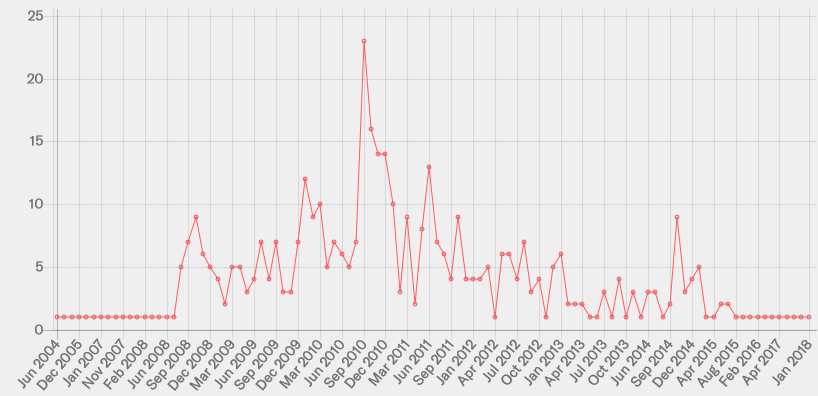
\includegraphics[width=\textwidth,height=\textheight,keepaspectratio]{Pakstrikes.png}
\end{figure}
\end{frame}

\begin{frame} 
	\frametitle{\LARGE{Casualties: 2,515-4,026 Dead}}
	\begin{figure}[ht!]
		\centering
		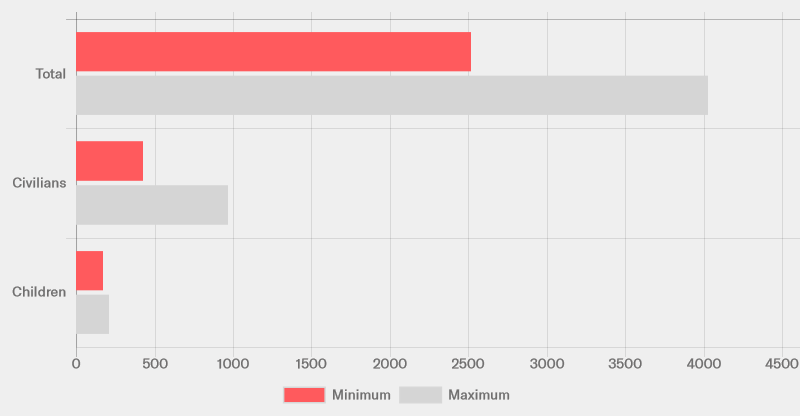
\includegraphics[width=\textwidth,height=\textheight,keepaspectratio]{Pakcas.png}
	\end{figure}
\end{frame}

\begin{frame} 
	\frametitle{\LARGE{Drone Strikes as Provocation}}
Known erroneous drone strikes across the entire program included: \pause
	\begin{itemize}
		\item Weddings \pause
		\item Funerals \pause
		\item Family gatherings \pause
		\item Farming activity \pause
	\end{itemize}
What does this look like? \textbf{The US playing right into a strategy of provocation by Al Qaeda.}
\end{frame}

\begin{frame} 
	\frametitle{\LARGE{Terrorism Summary 1}}
	\begin{itemize}
		\item Terrorism is a rational strategy. \pause
		\item The ultimate goal of a terror attack is to influence the general population beyond the immediate victims. \pause
		\item Terrorism is a strategy of weak, extremist groups that lack the numbers for civil war or legitimate political participation. \pause 
		\item Terrorist groups and states face acute bargaining issues.
	\end{itemize}
\end{frame}

\begin{frame} 
	\frametitle{\LARGE{Terrorism Summary 2}}
	\begin{itemize}
		\item Terrorism as a strategy of obtaining concessions is largely unsuccessful, and most terrorist groups fail. \pause
		\item While terrorism and civil war overlap, they are not synonymous.
		\item Terrorism can be used as a tactic for multiple aims: coercion, provocation, spoiling, and outbidding. \pause
		\item States have a variety of counterterrorism options, but must be wary of falling into a provocation trap.
	\end{itemize}
\end{frame}

\end{document}
